\documentclass[presentation]{beamer}
\usepackage{../oop-slides-pianini}
\setbeamertemplate{bibliography item}[text]
\newcommand{\lessonnr}[0]{06}
\title[OOP08 -- DCVS, GUI e IO]{08 \\ DVCS, parte II \\ Graphical User Interfaces e Input-Output}

\begin{document}

\frame[label=coverpage]{\titlepage}

%====================
%Outline
%====================
\begin{frame}<beamer>
 	\frametitle{Outline}
 	\tableofcontents[]
\end{frame}

\section{Decentralized Version Control Systems}

\subsection{Risolvere i merge conflict}

\fr{Conflicted files}{
	\bl{In generale}{
		Abbiamo visto nell'ultima lezione come sia possibile riunire due flussi di lavoro diversi.
		%
		Abbiamo anche visto che, nel caso in cui due linee di sviluppo abbiano modificato concorrentemente un file nello stesso punto, il merge non è banale da effettuare ma occorre risolvere manualmente un \emph{merge conflict}.
		
		In caso di merge conflict, l'operazione di merge non viene completata, e per tutti i file che presentano conflitti vengono creati:
		\iz {
			\item Un file .orig, che mostra il contenuto del file al momento della richiesta di merge
			\item Il file col nome precedente, contenente le linee di entrambe le teste.
		}
	}
}

\begin{frame}[fragile]{Esempio di conflict file}
	\begin{block}{}
		\tiny
		\begin{verbatim}
		public final class HelloWorld {
		private static final String AUTHOR = "Danilo Pianini";

		public static void main(final String[] args) {
		<<<<<<< local
			System.out.println("This program has been realised by " + AUTHOR);
		=======
			System.out.println("This program is running in a PC with " + procNumber() + " logic processors!");
		}

		public static int procNumber() {
			return Runtime.getRuntime().availableProcessors();
		>>>>>>> other
		}

		}
		\end{verbatim}
	\end{block}
\end{frame}

\fr{Merge strategies}{
	\bl{In generale}{
		I possibili modi per risolvere il conflitto sono:
		\iz {
			\item Conservazione del file .orig, ossia della release corrente. Si scartano le modifiche provenienti da altri branch.
			\item Editare il conflict file eliminando le righe non desiderate.
		}
		In ogni caso, al termine delle modifiche, è necessario dire al DVCS che il file è nello stato che desideriamo, marcando il conflitto come risolto, quindi procedere ad un \textit{commit}.
		
		La risoluzione del conflitto andrà applicata per ognuno dei file che stanno confliggendo con versioni parent.
	}
}

\fr{Errore frequente: bad tracking}{
	Cosa succede, se per errore abbiamo messo in tracking rigenerabili che non avremmo dovuto mettere?
	\bl{Un altro buon motivo per stare attenti a cosa si mette in tracking}{
		\begin{itemize}
		 \item Se abbiamo dei file binari in tracking (ad esempio dei class files che vengono ricompilati ogni volta), ad \textbf{ogni} merge avremo dei conflitti.
		 \item Ci sarà un conflitto per ogni risorsa modificata. Potenzialmente, centinaia ad ogni merge.
		 \item I conflitti su binari sono difficili da risolvere: il file può essere solo ispezionato tramite editor binari, e buona fortuna a capirne il contenuto.
		 \item Di norma si risolve cancellando tutti i file, rigenerandoli, marcando tutti i conflitti come risolti e facendo un commit.
		 \item \alert{\textbf{ESPLODE}} la dimensione del repository
		 \item State attenti a cosa mettete in tracking!
		\end{itemize}
	}
}

\fr{Merge strategies}{
	\bl{Conservazione del file .orig In Mercurial}{
		Supponendo di essere nel branch \texttt{default} e di voler mergere in questo branch il branch \texttt{feature}, e supponendo che il nome del file in conflitto sia \texttt{file1}:
		\begin{enumerate}
			\item Chiediamo a Mercurial di risolvere automaticamente il maggior numero possibile di conflitti
			\begin{itemize}
				\item \texttt{hg merge feature}
			\end{itemize}
			\item Rimuoviamo il file confliggente
			\begin{itemize}
				\item \texttt{hg rm file1}
			\end{itemize}
			\item Rinominiamo il file originale che vogliamo mantenere
			\begin{itemize}
				\item \texttt{hg mv file1.orig file1}
			\end{itemize}
			\item Il conflitto è risolto, informiamo Mercurial della cosa
			\begin{itemize}
				\item \texttt{hg resolve -m file1}
				\item L'opzione \texttt{-m} nel comando \texttt{resolve} sta per ``mark''
			\end{itemize}
			\item Conflitto risolto, possiamo fare il merge commit
			\begin{itemize}
				\item \texttt{hg commit}
			\end{itemize}
		\end{enumerate}
	}
}

\fr{Merge strategies}{
	\bl{Modifica del conflict file in Mercurial}{
		Supponendo di essere nel branch \texttt{default} e di voler mergere in questo branch il branch \texttt{feature}, e supponendo che il nome del file in conflitto sia \texttt{file1}:
		\begin{enumerate}
			\item Chiediamo a Mercurial di risolvere automaticamente il maggior numero possibile di conflitti
			\begin{itemize}
				\item \texttt{hg merge feature}
			\end{itemize}
			\item Rimuoviamo il file originale (non via \texttt{hg}: non è in tracking!)
			\begin{itemize}
				\item \texttt{rm file1.orig}
			\end{itemize}
			\item Apriamo con un editor di testo \texttt{file1}, e lo modifichiamo fin quando non ha l'aspetto che vorremmo.
			\item Il conflitto è risolto, informiamo Mercurial della cosa
			\begin{itemize}
				\item \texttt{hg resolve -m file1}
				\item L'opzione \texttt{-m} nel comando \texttt{resolve} sta per ``mark''
			\end{itemize}
			\item Conflitto risolto, possiamo fare il merge commit
			\begin{itemize}
				\item \texttt{hg commit}
			\end{itemize}
		\end{enumerate}
	}
}



\subsection{Lavorare in gruppo: clone, pull, push}

\fr{Decentralizzazione}{
	\bl{Decentralizzazione totale...}{
		Nei DVCS, non esiste un punto centrale che fa repository ``ufficiale'': tutti i repository ricevono l'intera storia ed hanno pari importanza.
		
		Il design dei DVCS è ideale per un mondo P2P
	}
	\bl{... nella realtà della struttura di Internet}{
		Per via della struttura attuale di Internet, della presenza di NAT e simili strutture di rete, il modello client/server è spesso difficile da aggirare.
		%
		È spesso anche sconveniente aggirarlo: tutto sommato, il cloud spesso è utile...
		
		Esistono servizi di hosting che consentono di avere in un punto sempre accessibile dei repository in rete: chi ha bisogno di collaborare non deve preoccuparsi di problematiche di rete diverse da ``andare sul web''.
	}
}

\fr{Clone}{
	\bl{In generale}{
		Occorre un meccanismo che consenta di fare copie di repository esistenti, al fine di cominciare a lavorare su qualcosa di già esistente, o di effettuare copie di sicurezza del proprio lavoro.
	}
	\bl{In Mercurial}{
		\iz{
			\item \texttt{hg clone URI localfolder}
		}
		Scarica l'intera storia del repository conservato in \texttt{URI} all'interno di \texttt{localfolder}, che diventa un repository Mercurial. Esempi di \texttt{URI}:
		\iz {
			\scriptsize
			\item \texttt{/home/user/repository/} --- URI locale (*nix)
			\item \texttt{C:\textbackslash{}Users\textbackslash{}Username\textbackslash{}repository\textbackslash{}} --- URI locale (Windows)
			\item \texttt{file://home/user/repository/} --- URI locale con protocollo file (Unix)
			\item \texttt{ssh://username@server/repository/} --- URI Secure Shell (raccomandata per chi lavora in remoto con server e/o client *nix)
			\item \texttt{https://user@server/repository/} --- URI HTTPS, multipiattaforma
		}
	}
}

\fr{Default remote repository}{
	\bl{In generale}{
		Al momento del clone, vogliamo conservare un riferimento a quale sia la sorgente iniziale da cui abbiamo preso il codice.

		In caso di operazioni remote, infatti, è comodo avere un riferimento da cui leggere eventuali nuovi commit o sui cui scrivere i nostri commit.
	}
	\bl{In Mercurial}{
		Al momento del \texttt{clone}, le informazioni circa il repository da cui si è effettuata la copia vengono conservate nel file \texttt{.hg/hgrc} all'interno del repository. Nel file viene creata un'opzione \texttt{[paths]} e alla variabile \texttt{default} viene assegnato il valore dell'URI che abbiamo clonato.

		È possibile modificare il file suddetto per modificare quale sia il repository default.
	}
}

\begin{frame}[fragile]{Esempio di \texttt{.hg/hgrc} dopo \texttt{hg clone}}
	\begin{block}{}
		\begin{verbatim}
			[paths]
			default = ssh://hg@bitbucket.org/danysk/test
		\end{verbatim}
	\end{block}
\end{frame}

\fr{Pull}{
	\bl{In generale}{
		Vogliamo una operazione che ci consenta di acquisire nuovi commit da una fonte, in maniera tale da acquisire il lavoro fatto da altri. Tale operazione si chiama pull, e \emph{teoricamente} è l'unica operazione necessaria a rendere completamente distribuito un DVCS.
	}
	\bl{In Mercurial}{
		\iz{
			\item \texttt{hg pull URI}
			\item \texttt{hg pull}
		}
		Il comando suddetto scarica tutti i commit di \texttt{URI} e li integra nel repository corrente. Dopo l'operazione di pull, per aggiornare i file alla versione scaricata è necessario \texttt{hg update}. È possibile che vengano aggiunte nuove teste al repository, nel qual caso è possibile effettuare una operazione di merge. Se \texttt{URI} viene omesso, viene utilizzato il valore della variabile \texttt{default} nel file \texttt{.hg/hgrc}. Se tale valore non è presente, la pull fallisce.
	}
}

\fr{Esempio con \texttt{clone} e \texttt{pull}}{
  Situazione iniziale \\
  \begin{center}
    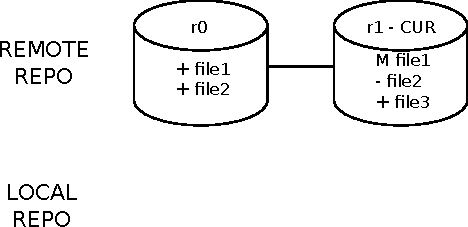
\includegraphics[width=0.99\textwidth]{img/draw3}
  \end{center}
}

\fr{Esempio con \texttt{clone} e \texttt{pull}}{
  Local esegue:\\
  \texttt{hg clone indirizzo\_di\_remote\_repo} \\
  \begin{center}
    \includegraphics[width=0.8\textwidth]{img/draw4}
  \end{center}
}

\fr{Esempio con \texttt{clone} e \texttt{pull}}{
  Local esegue:\\
  modifica di \texttt{file3} \\
  \texttt{commit} \\
  \begin{center}
    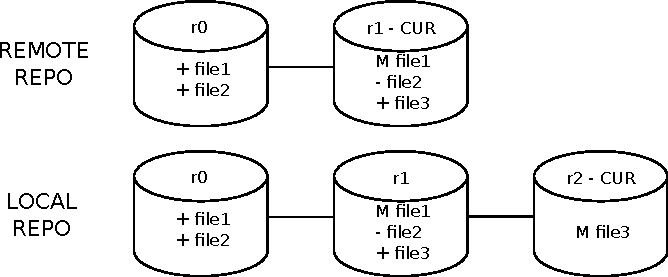
\includegraphics[width=0.99\textwidth]{img/draw5}
  \end{center}
}

\fr{Esempio con \texttt{clone} e \texttt{pull}}{
  Remote esegue:\\
  \texttt{hg pull indirizzo\_di\_local\_repo} \\
  \texttt{update r2} \\
  \begin{center}
    \includegraphics[width=0.99\textwidth]{img/draw6}
  \end{center}
}

\fr{Push}{
	\bl{In generale}{
		Nella realtà dei fatti l'operazione di pull non è sufficiente: si pensi ad esempio se volessimo far sì che un server pull-asse alcuni nostri commit, ma non avessimo accesso al suddetto, o non fossimo raggiungibili. L'operazione duale della \texttt{pull} si chiama \texttt{push}, ed è più delicata: chi la esegue deve avere i diritti di scrittura verso la destinazione.
	}
	\bl{In Mercurial}{
		\iz{
			\item \texttt{hg push URI}
			\item \texttt{hg push}
		}
		\scriptsize
		Il comando suddetto carica tutti i commit del repository corrente nel repository presente in \texttt{URI}. Dopo l'operazione di push, per aggiornare i file alla versione caricata è necessario eseguire \texttt{hg update} sulla destinazione. È possibile configurare il repository destinazione per eseguire automaticamente l'operazione. Se \texttt{URI} viene omesso, viene utilizzato il valore della variabile \texttt{default} nel file \texttt{.hg/hgrc}. Se tale valore non è presente, la push fallisce.
	}
}

\begin{frame}{Push di un nuovo branch}
	\begin{block}{Creazione e push di un nuovo branch}
		Qualora il nostro nuovo commit creasse un nuovo branch, la \texttt{push} viene normalmente rifiutata, col messaggio:
		
		\texttt{abort: push creates new remote branches: BRANCHNAME!}
		
		Per poter \texttt{push}-are un nuovo branch, è necessario utilizzare esplicitamente l'opzione \texttt{--new-branch}.
	\end{block}
\end{frame}

\begin{frame}{Push e multihead}
	\begin{block}{Multiple heads}
		Qualora il nostro nuovo commit creasse un una nuova linea di sviluppo, la \texttt{push} verrà normalmente rifiutata, col messaggio:
		
		\texttt{abort: push creates new remote heads!}
		
		È \textbf{fortemente} sconsigliato lavorare in multi-head su un singolo branch. Il modo corretto di portare a termine l'operazione non è quello di forzare la \texttt{push} (usando un'opzione che \emph{non} vi verrà detta), ma:
		\begin{itemize}
			\item Se la creazione della nuova linea di sviluppo è voluta, va creato un ``named branch'', e ci si riporta al caso precedente.
			\item Se la creazione della nuova linea di sviluppo non è voluta, si effettua un merge delle teste del branch corrente, e si effettua una \texttt{push} normale.
		\end{itemize}
	\end{block}
\end{frame}


\fr{Esempio con \texttt{push}}{
  Situazione iniziale:
  \begin{center}
    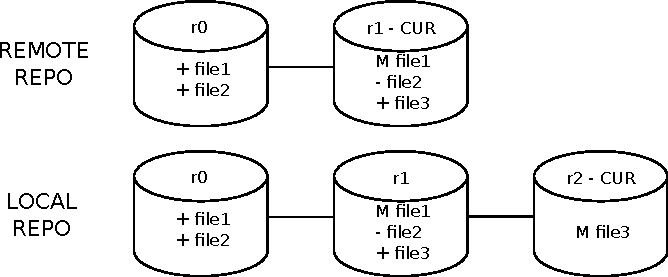
\includegraphics[width=0.99\textwidth]{img/draw5}
  \end{center}
}

\fr{Esempio con \texttt{push}}{
  Local esegue: \texttt{hg push indirizzo\_di\_remote\_repo} \\
  Remote esegue: \texttt{hg update} \\
  \begin{center}
    \includegraphics[width=0.99\textwidth]{img/draw6}
  \end{center}
}


\fr{Lavorare in parallelo: esempio}{
  Situazione iniziale:
  \begin{center}
    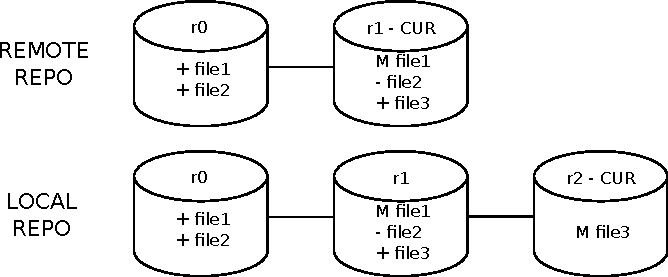
\includegraphics[width=0.99\textwidth]{img/draw5}
  \end{center}
}

\fr{Lavorare in parallelo: esempio}{
  Remote esegue:\\
  Modifica di \texttt{file2} \\
  \texttt{hg commit} \\
  \begin{center}
    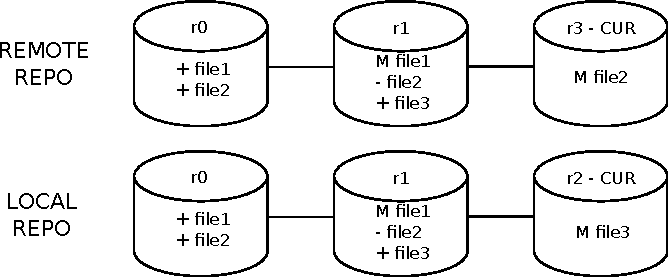
\includegraphics[width=0.99\textwidth]{img/draw7}
  \end{center}
}

\fr{Lavorare in parallelo: esempio}{
  Local esegue:\\
  \texttt{hg push indirizzo\_di\_remote\_repo} \\
  \begin{center}
    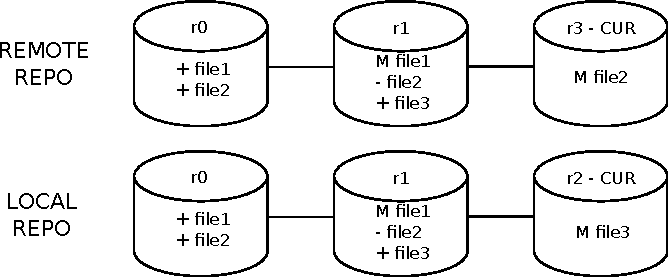
\includegraphics[width=0.99\textwidth]{img/draw7}
  \end{center}
  La push viene rifiutata: la radice dei due repository è diversa!
}

\fr{Lavorare in parallelo: esempio}{
  Local esegue:\\
  \texttt{hg pull indirizzo\_di\_remote\_repo} \\
  \begin{center}
    \includegraphics[width=0.7\textwidth]{img/draw8}
  \end{center}
  Il repository locale ora può essere portato anche alla versione \texttt{r3}. Nonostante ciò, le push (a meno di utilizzare l'opzione \texttt{--force}) vengono rifiutate, poiché il repository locale ha due teste!
}

\fr{Merge: esempio}{
  Local esegue:\\
  \texttt{hg merge} \\
  \texttt{hg commit} \\
  \begin{center}
    \includegraphics[width=0.99\textwidth]{img/draw9}
  \end{center}
  Ora è possibile effettuare push: c'è una sola testa!
}

\fr{Merge: esempio}{
  Local esegue:\\
  \texttt{hg push indirizzo\_di\_remote\_repo} \\
  \begin{center}
    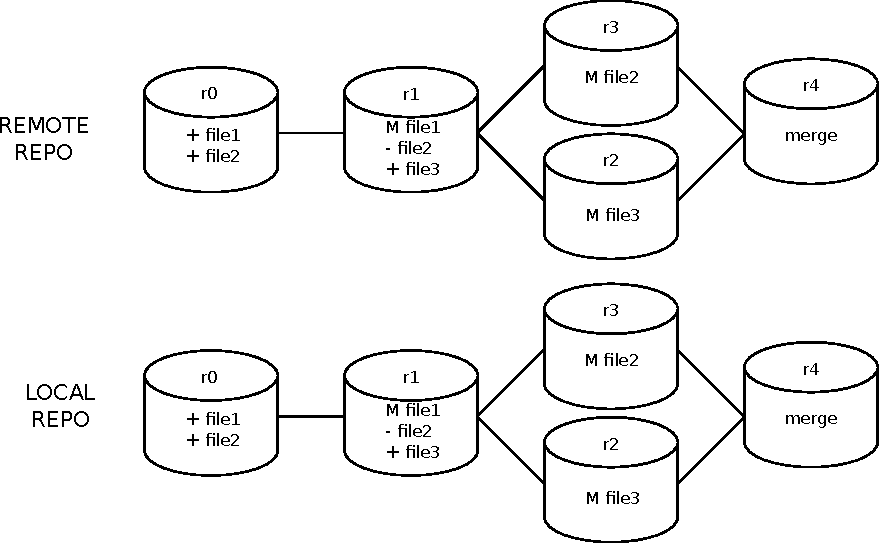
\includegraphics[width=0.8\textwidth]{img/draw10}
  \end{center}
  Ora è possibile effettuare push: c'è una sola testa!
}

\subsection{Hosting e Bitbucket}

\fr{Bitbucket Overview}{
	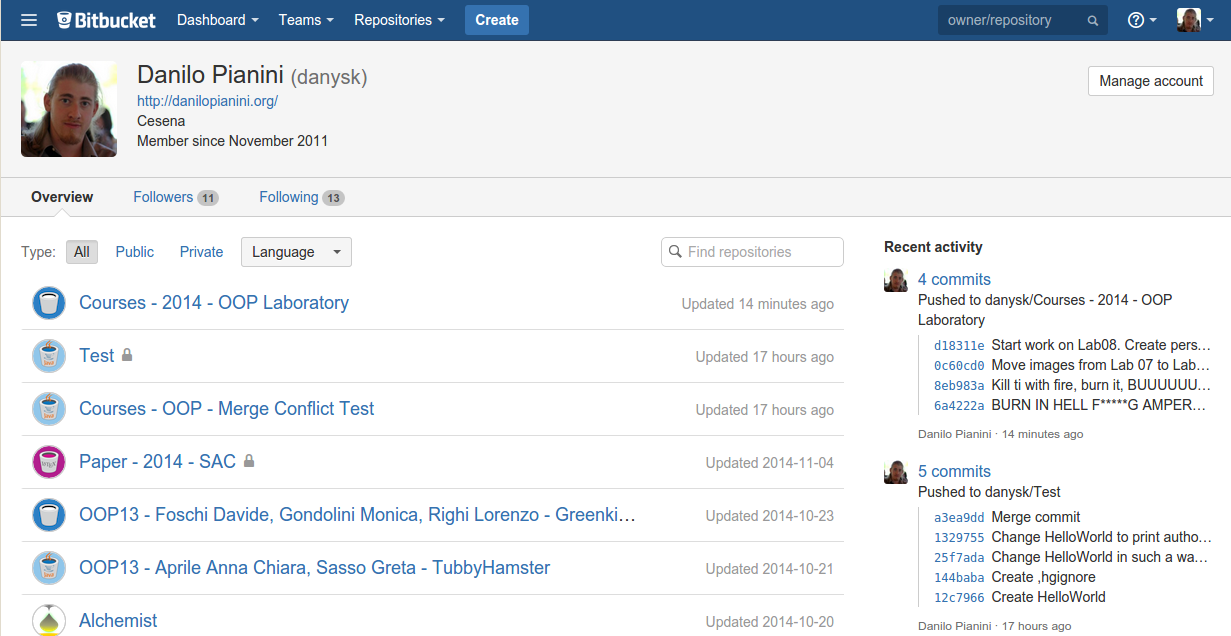
\includegraphics[width=0.99\textwidth]{img/bitbucket0}
}

\fr{Bitbucket Overview}{
	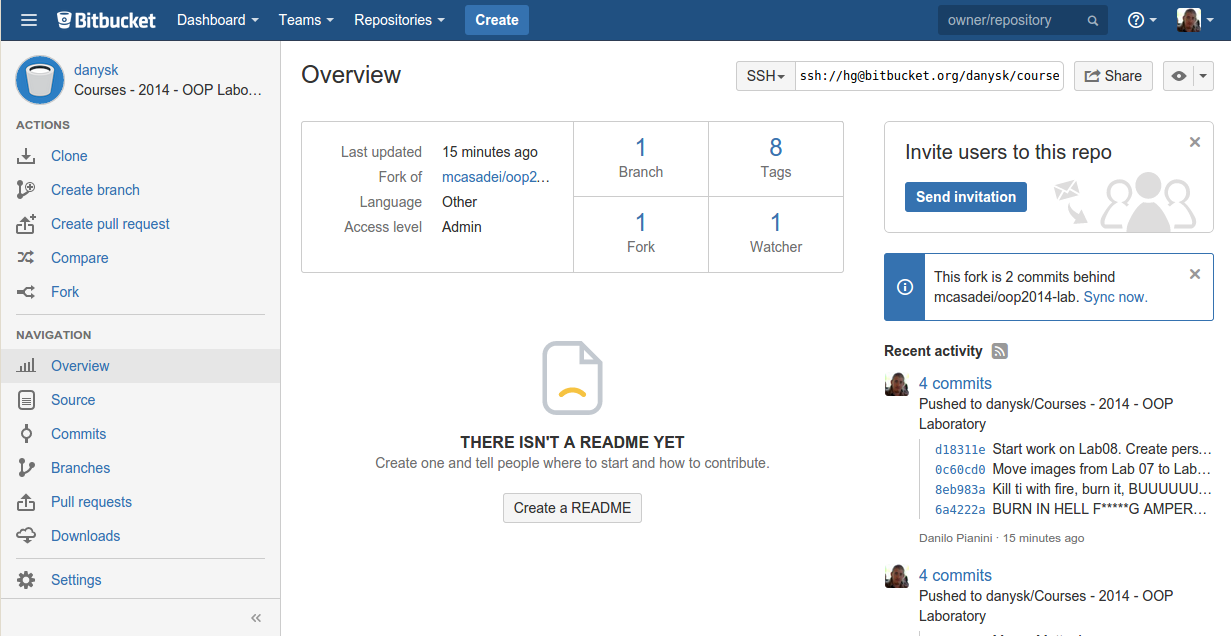
\includegraphics[width=0.99\textwidth]{img/bitbucket1}
}

\fr{Bitbucket Overview}{
	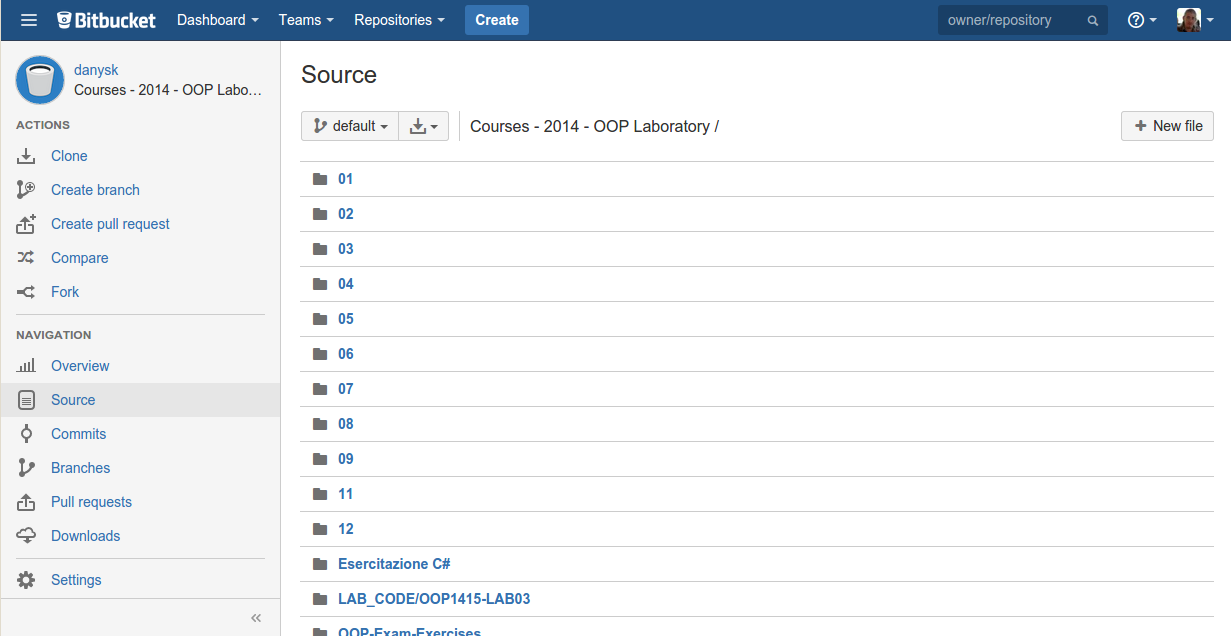
\includegraphics[width=0.99\textwidth]{img/bitbucket2}
}

\fr{Bitbucket Overview}{
	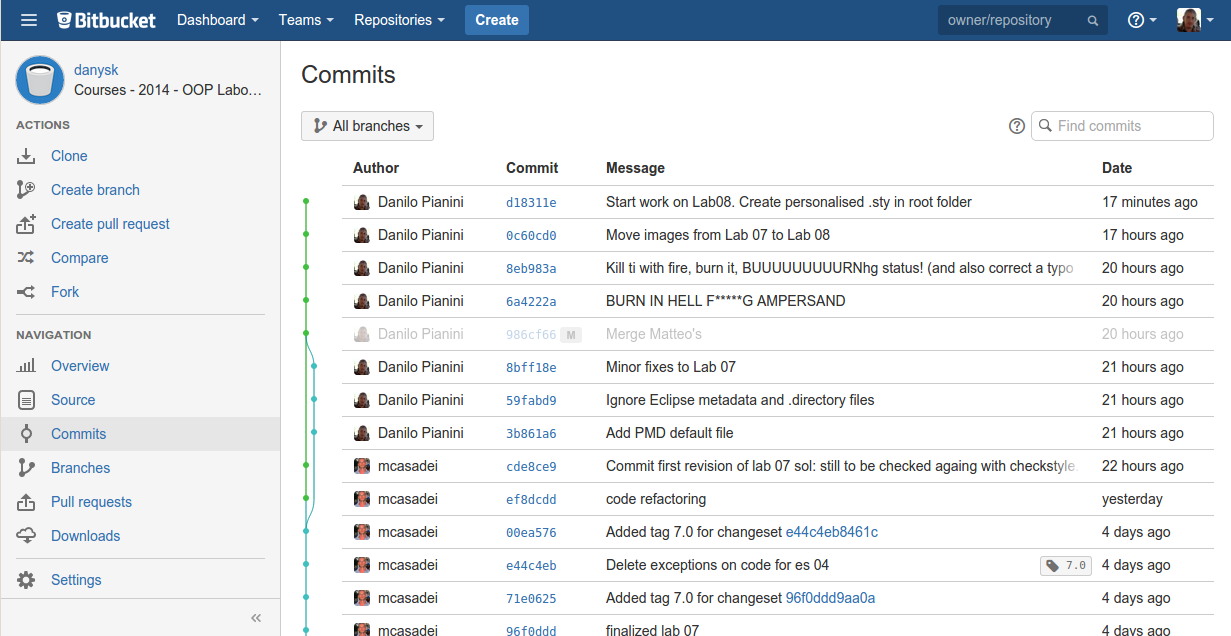
\includegraphics[width=0.99\textwidth]{img/bitbucket3}
}

\fr{Bitbucket Overview}{
	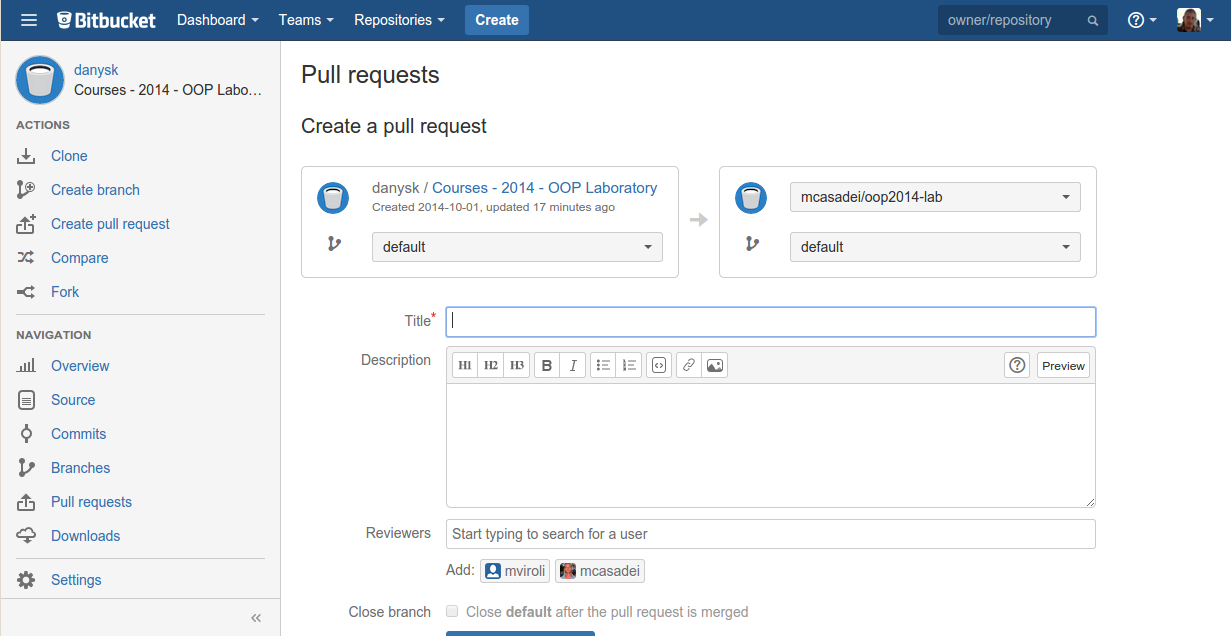
\includegraphics[width=0.99\textwidth]{img/bitbucket4}
}

\fr{Bitbucket Overview}{
	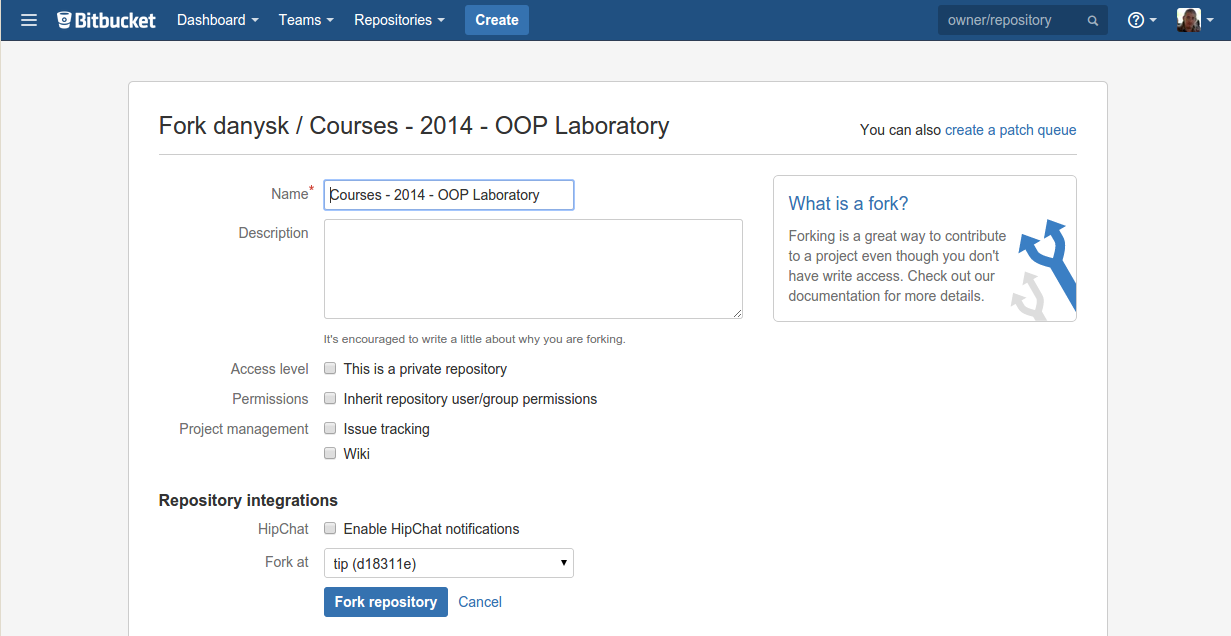
\includegraphics[width=0.99\textwidth]{img/bitbucket5}
}

\fr{Bitbucket Overview}{
	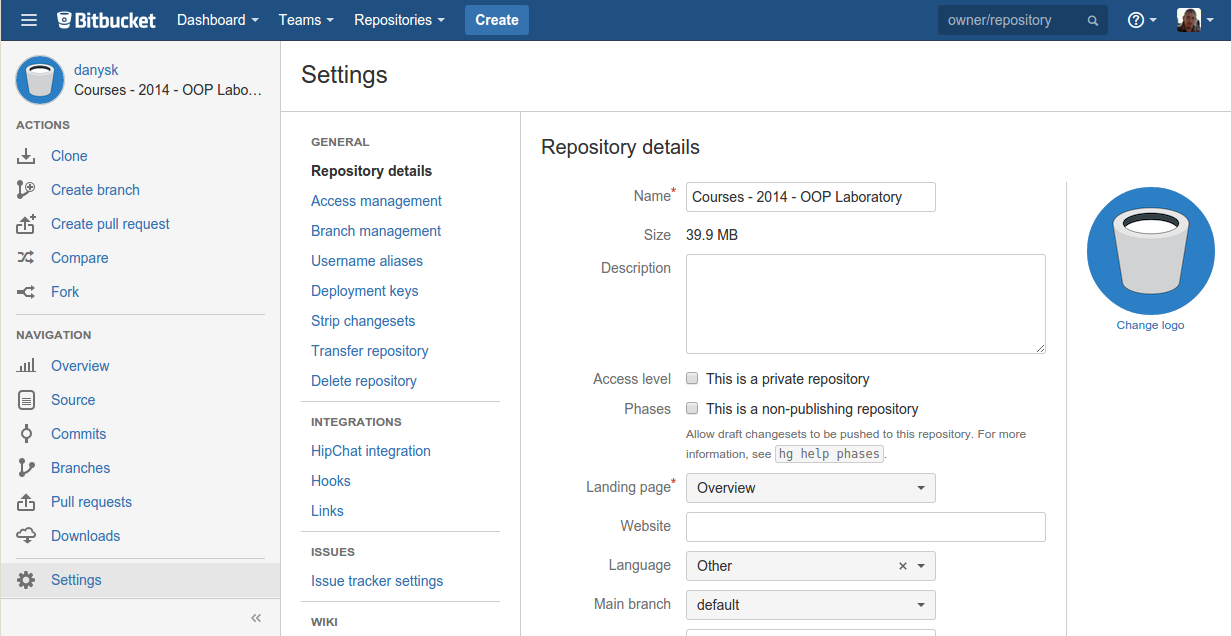
\includegraphics[width=0.99\textwidth]{img/bitbucket6}
}

\fr{Bitbucket Overview}{
	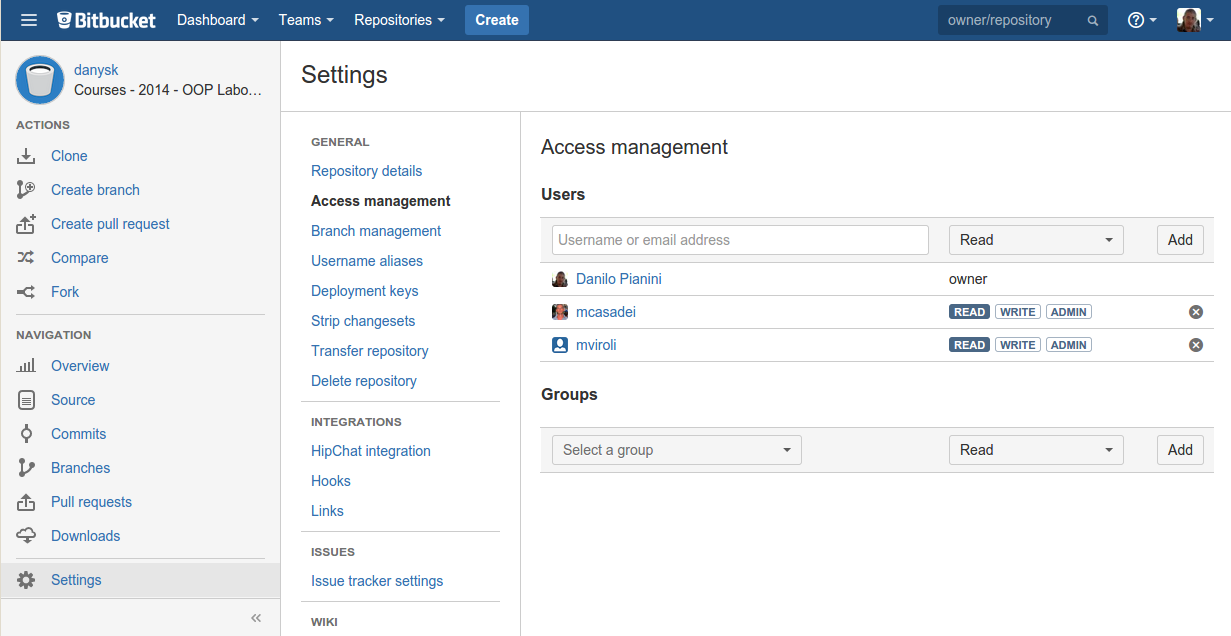
\includegraphics[width=0.99\textwidth]{img/bitbucket7}
}

\fr{Bitbucket Overview}{
	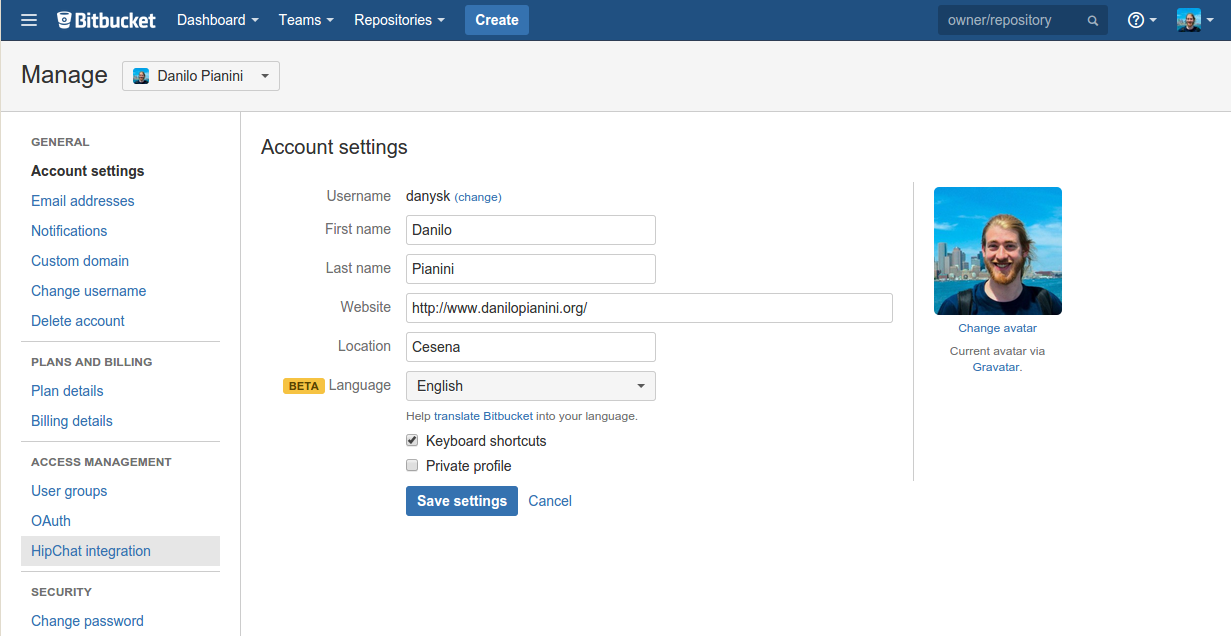
\includegraphics[width=0.99\textwidth]{img/bitbucket9}
}

\fr{Bitbucket Overview}{
	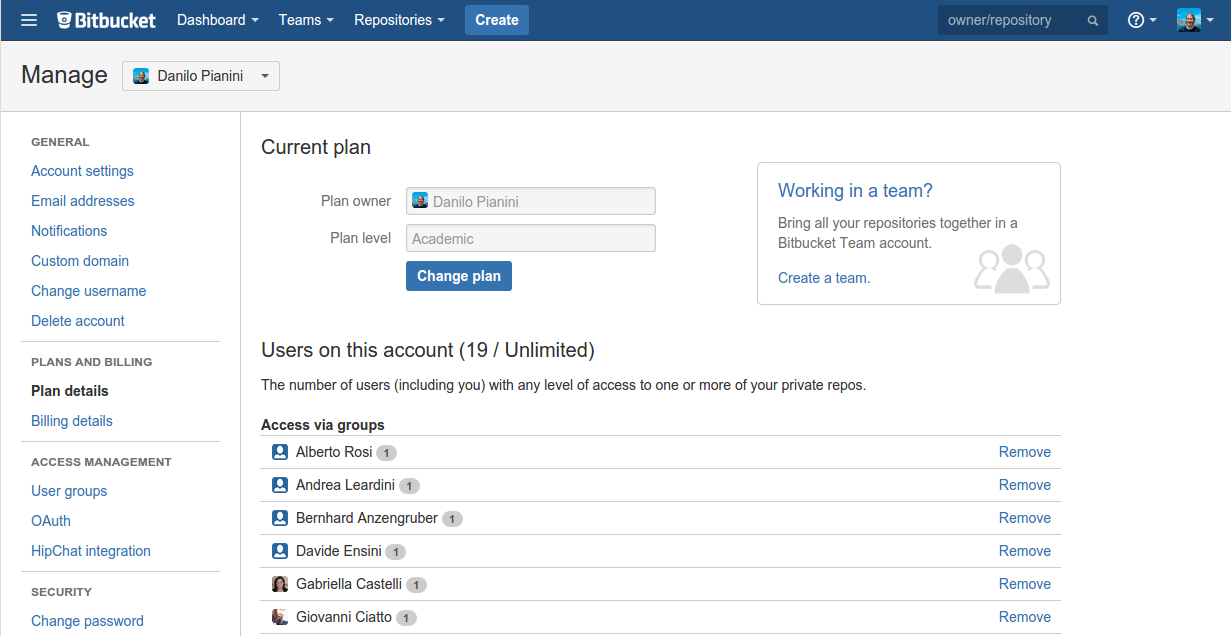
\includegraphics[width=0.99\textwidth]{img/bitbucket10}
}

\fr{Bitbucket Overview}{
	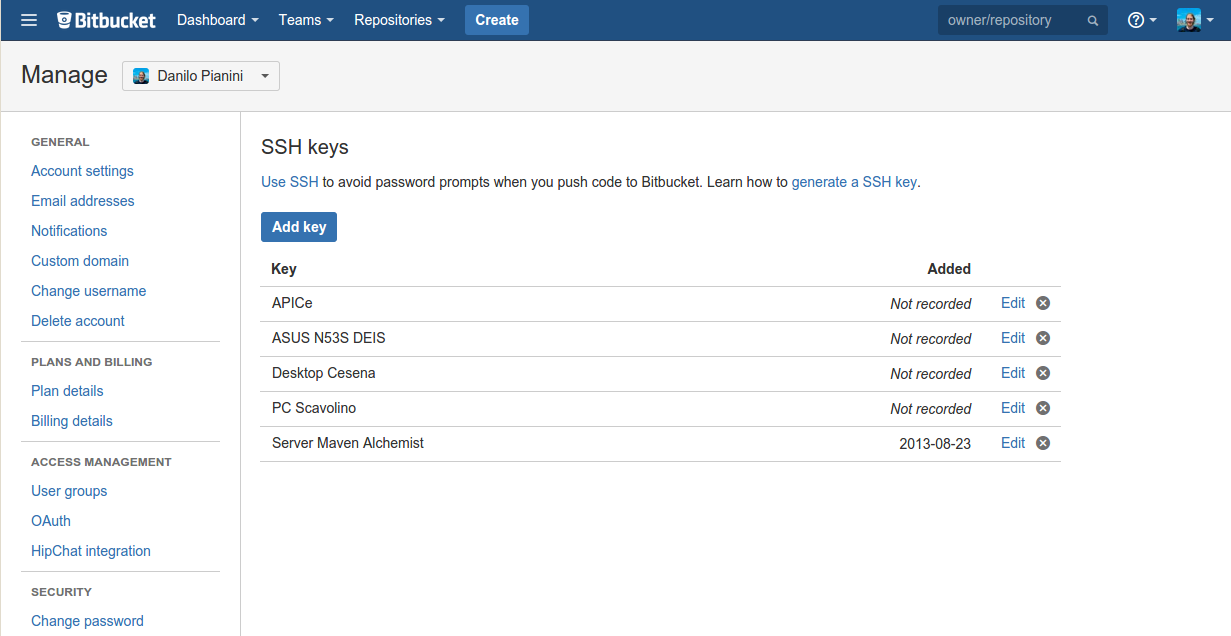
\includegraphics[width=0.99\textwidth]{img/bitbucket11}
}

\fr{Bitbucket Overview}{
	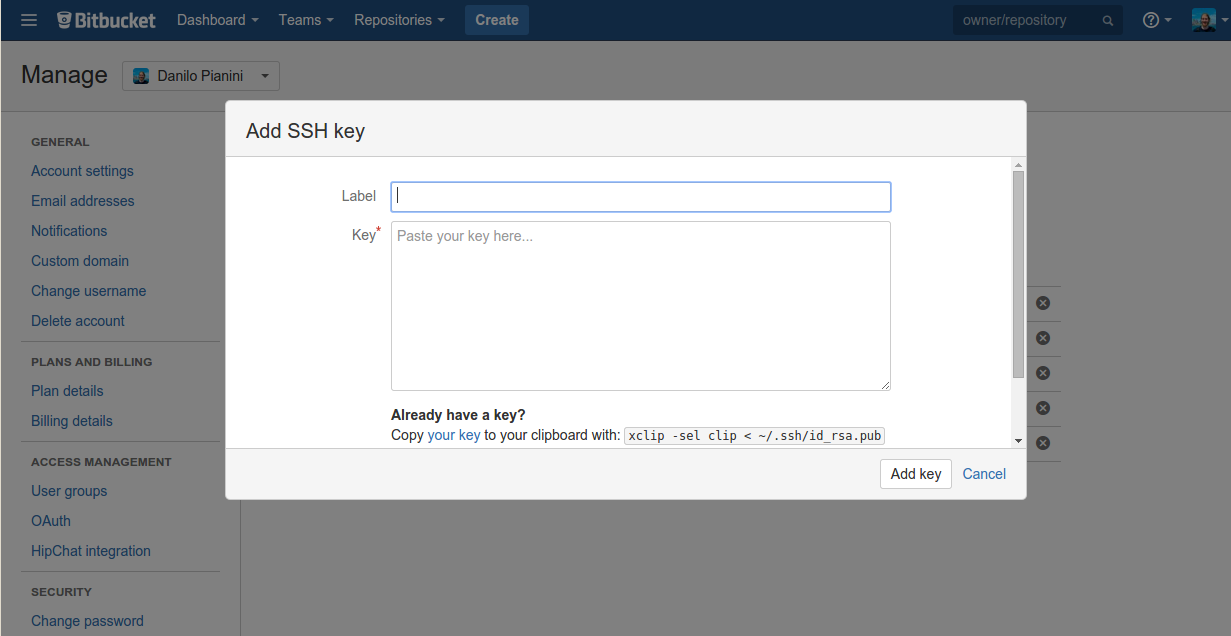
\includegraphics[width=0.99\textwidth]{img/bitbucket12}
	
	\scriptsize
	Su sistemi *nix, si utilizzi il comando \texttt{ssh-keygen -t rsa} per generare una coppia di chiavi pubblica e privata. Non si inserisca alcuna password e si mantengano le opzioni suggerite dal sistema. A questo punto, all'interno della cartella \texttt{\textasciitilde{}/.ssh/}, si troveranno i file delle chiavi. Si incolli nel campo key il contenuto del file \texttt{\textasciitilde{}/.ssh/id\_rsa.pub}

}

\subsection{Plugin Eclipse (MercurialEclipse - HGE)}

\fr{Plugin eclipse}{
	\bl{Installazione}{
		Il plugin può essere installato tramite il marketplace di Eclipse. Le istruzioni sono disponibili nella pagina per l'installazione del software del corso.
	}
	\bl{Funzionalità}{
		Il plugin HGE mostrerà le proprie funzionalità dal menu ``Team'', ed esporrà le stesse funzionalità del tool a linea di comando, \alert{più altre che non dovete utilizzare se non avete \textbf{cristallino} il loro funzionamento da terminale}.

		È anche possibile utilizzare il menu Import $\rightarrow$ Mercurial $\rightarrow$ Clone Existing Mercurial repository.
	}
}

\begin{frame}{Quando usare il plugin}
	È bene (come per tutte le utility con interfaccia grafica) fare un utilizzo \textbf{consapevole} del plugin Eclipse.
	
	Di seguito alcuni consigli per la gestione di progetti, che potete violare a vostro rischio e pericolo:
	
	\begin{block}{Quando è meglio utilizzare il plugin Eclipse}
		\begin{itemize}
			\item In caso di cancellazione o refactoring (rinominazioni): il plugin rinomina e cancella chiamando in automatico hg mv e hg rm, e conseguentemente è più semplice utilizzarlo rispetto all'equivalente da terminale
			\item In caso di merge conflict, il plugin fornirà una vista dei file in conflitto e, per ciascuno, mostrerà le differenze fra il file originale e quello che si desidera mergere. Una volta che nella colonna di sinistra appare il file così come lo si desidera, è possibile marcare il conflitto come risolto.
		\end{itemize}
	\end{block}
	
	Per le restanti operazioni, si caldeggia l'uso del tool da terminale.
	
	\textbf{Ogni} altro tool per la gestione di Mercurial via GUI è sconsigliato.
\end{frame}

\end{document}

\subsection{Workflow}

\fr{Shared repository}{
  \iz {
    \item Funziona bene se:
    \iz {
      \item Il progetto è piccolo
      \item Ci sono pochi membri nel team
      \item I membri del team possono interagire con facilità
      \item Non c'è un maintainer/leader vero e proprio
    }
    \item Come funziona:
    \iz {
      \item Un solo repository online ``di riferimento''
      \item Tutti i membri fanno pull e push su quello
    }
    \item Regole per farlo funzionare bene:
    \iz {
      \item Ciascun membro deve fare pull prima di fare push
      \item Nel caso in cui la pull richieda di eseguire un'operazione di merge, è responsabilità di chi ha fatto la pull eseguire il merge correttamente prima di fare push
    }
    \item Difetti:
    \iz {
      \item Un solo membro che lavora male può compromettere il repository
      \item Gara a chi fa push per primo per evitare di dover eseguire i merge
    }
  }
}

\fr{Shared repository}{
  \begin{center}
    \includegraphics[width=0.99\textwidth]{img/shared}
  \end{center}
}

\fr{Multiple forks and pull requests}{
  \iz {
    \item Funziona bene se:
    \iz {
      \item Il progetto è grande
      \item I membri del team non riescono a tenersi in contatto, ad esempio perché non lavorano nello stesso ufficio
      \item C'è un maintainer o un responsabile
    }
    \item Come funziona:
    \iz {
      \item Un repository online ``di riferimento'', gestito dal maintainer
      \item Ogni sviluppatore fa una fork del repository principale
      \item Gli sviluppatori pull-ano dal repository principale e push-ano sulla loro fork
      \item Quando la funzionalità che si voleva integrare è pronta per la consegna, lo sviluppatore apre una pull request verso il main repo
      \item Il maintainer può analizzare il codice che verrebbe modificato, se accetta le modifiche il main repo viene portato nello stesso stato della fork.
    }
    \item Regole per farlo funzionare bene:
    \iz {
      \item Il maintainer deve essere in grado di effettuare code review
    }
    \item Difetti:
    \iz {
      \item Più complicato di un singolo repository condiviso
    }
  }
}

\fr{Multiple forks and pull requests}{
  \begin{center}
    \includegraphics[width=0.99\textwidth]{img/forks}
  \end{center}
}

\subsection{Features avanzate}

\fr{Aspetti avanzati}{
  \bl{Rebasing}{
    Procedura alternativa al merge, in cui i due commit, invece di essere fusi, vengono messi in sequenza.
  }
  \bl{Cherry picking}{
    Pull di un singolo commit o di un piccolo gruppo di commit. Spesso utilizzato quando si desidera avere un bugfix che si trova in un altro branch, ma non tutto il resto. Molto comune nel backporting delle patch di sicurezza.
  }
  \bl{Bisection}{
    Strategia per scoprire bug in maniera automatizzata, testando il software a varie versioni (ricerca dicotomica). Una volta trovata la prima versione dove il bug si verifica, si controllano commit message e le differenze.
  }
}



\fr{Esercizio con Mercurial} {
	\iz{
		\item Si acceda a \url{https://bitbucket.org/}
		\item Ci si logghi con il proprio utente
		\item Si vada al progetto che si trova alla pagina \url{https://bitbucket.org/danysk/courses-oop-merge-conflict-test}
		\item Dall'interfaccia web di Bitbucket, si crei una propria fork del progetto
		\item Utilizzando il comando \texttt{hg clone}, si cloni \textbf{la propria fork del progetto} all'interno di una nuova directory
		\item Utilizzando il comando \texttt{hg heads}, si verifichi che il progetto ha due teste
		\item Si tenti di fare il merge utilizzando \texttt{hg merge} 
		\item Si osservi l'output di Mercurial: il merge ha generato un conflitto
		\item Si utilizzi il comando \texttt{ls -ahl} (su Windows si usi l'equivalente \texttt{dir}) per vedere l'elenco dei file
		\item Si noti che è stato creato un file \texttt{.origin}
	}
}

\fr{Esercizio con Mercurial} {
	\iz{
		\item Utilizzando il comando \texttt{cat} (in Windows si usi il comando equivalente \texttt{type}) si osservi il contenuto dei file \texttt{HelloWorld.java.orig} e \texttt{HelloWorld.java}
		\item Si modifichi HelloWorld.java in modo che stampi le informazioni riguardanti l'autore (non si modifichi l'autore al momento) e che stampi nella linea successiva l'informazione sul numero di processori installati.
		\item Si compili nella cartella \texttt{bin} il file \texttt{HelloWorld.java}
		\item Se ne testi il funzionamento
		\item Una volta che il programma è funzionante, si usi hg status per vedere lo stato del repository. Si noti che il file \texttt{.orig} è in stato \texttt{?}
		\item Si elimini il file \texttt{.orig}
		\item Si dichiari risolto il conflitto di merge di \texttt{HelloWorld.java} utilizzando propriamente il comando \texttt{hg resolve -m}
		\item Si salvi il merge con \texttt{hg commit}
	}
}

\fr{Esercizio con Mercurial} {
	\iz{
		\item Dall'interfaccia web di Bitbucket, si crei un nuovo repository online
		\item Si faccia \texttt{hg push} del repository locale verso il nuovo repository online
		\item Si osservi, nell'interfaccia web di Bitbucket, la storia dei commit ed il grafo che mostra l'evoluzione dei flussi di lavoro
		\item Si modifichi \texttt{HelloWorld.java} in modo tale che stampi il nome e cognome dello studente
		\item Si esegua commit
		\item In una nuova cartella \textbf{fuori dal repository corrente}, si cloni la precedente fork del repository (che avrà ancora le due teste separate)
		\item Si modifichi il file \texttt{.hg/hgrc} facendo sì che punti al nuovo repository creato su Bitbucket
		\item Si eseguano \texttt{hg pull} e \texttt{hg update}
		\item Si verifichi con \texttt{hg log} e \texttt{hg heads} che il nuovo repository locale ha incorporato le modifiche fatte in precedenza. 
	}
}


